\chapter{統計グラフ入門}


\section{matplotlib入門}
pythonでグラフを書く時の最も有名なライブラリはmatplotlibといわれるものを利用します。

matplotlibの基本的な利用方法を確認しましょう。

\subsection{matplotlibの使い方}
matplotlibライブラリの中のpyplot(データプロットモジュール)を利用します。この時にimportは「matplotlib.pyplot」となるので利用する際のライブラリ名と機能名の名称が長くなるためasによって別名をつけることが一般的です。

\begin{verbatim}
import matplotlib.pyplot as plt

\end{verbatim}

\begin{hipoint}{Point}
matplotlibライブラリを利用するには次のコマンドでpythonのmatplotlibライブラリをインストールする必要があります。
\begin{verbatim}
pip install matplotlib
\end{verbatim}
\end{hipoint}
\subsection{グラフの描画と表示}
グラフに描画するためのデータを用意して表示してみましょう。

\newpage
\begin{pabox}{graph-1(折れ線グラフ)}
6要素のデータ[100,50,200,300,350,500]の折れ線グラフを描画してみましょう。
基本的なグラフはx軸の値とy軸の値を指定することで簡単に表示することができます。
\begin{legbox}{class1-1.py}
\begin{listing}{1}
import matplotlib.pyplot as plt

x = [ 1, 2, 3, 4, 5, 6 ]
data = [ 100, 50, 200, 300, 350, 500 ]
plt.plot( x, data )
#plotを使ってデータを指定します。
plt.show()
\end{listing}


実行結果\\

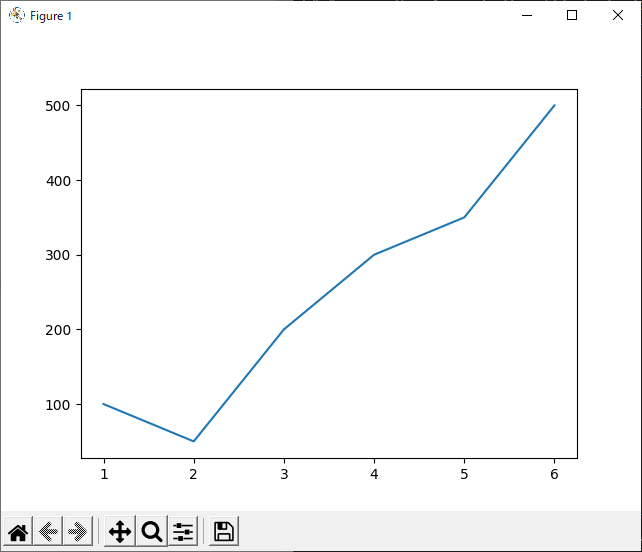
\includegraphics[width=7cm]{images/graph1.png} 

\end{legbox}
\end{pabox}
\newpage

\begin{pabox}{graph-2(棒グラフ)}
6要素のデータ[200,220,240,220,260,210]の棒グラフを描画してみましょう。
基本的なグラフはx軸の値とy軸の値を指定することで簡単に表示することができます。
\begin{legbox}{class1-2.py}
\begin{listing}{1}
import matplotlib.pyplot as plt

x = [ 1, 2, 3, 4, 5, 6 ]
data = [ 200, 220, 240, 220, 260, 210 ]

plt.bar( x, data )
#barを使ってデータを指定します。
plt.show()
\end{listing}


実行結果\\

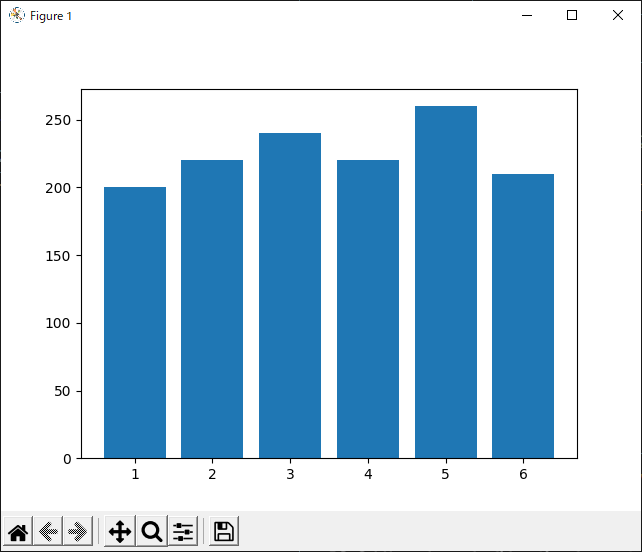
\includegraphics[width=7cm]{images/graph2.png} 

\end{legbox}
\end{pabox}

\newpage
\begin{pabox}{graph-3(円グラフ)}
6要素のデータ[100,200,300,400,500,600]の円グラフを描画してみましょう。
\begin{legbox}{graph1-3.py}
\begin{listing}{1}
import matplotlib.pyplot as plt

data = [ 100, 200, 300, 400, 500, 600 ]
plt.pie( data )
#pieを使ってデータを指定します。
plt.show()
\end{listing}


実行結果\\

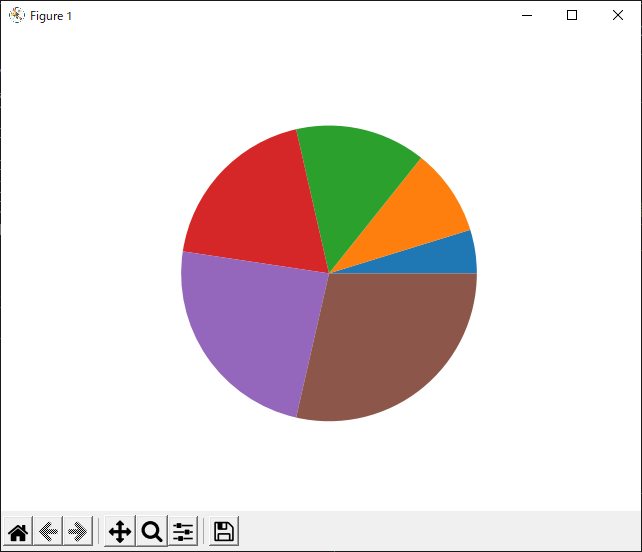
\includegraphics[width=7cm]{images/graph3.png} 

\end{legbox}
\end{pabox}
\newpage
\begin{pabox}{graph-4(データラベル)}
graph-2の棒グラフのデータラベルに日本語でラベルを設定してみましょう。
\begin{legbox}{graph1-4.py}
\begin{listing}{1}
import matplotlib.pyplot as plt
import japanize_matplotlib
#日本語matplotlibを設定

x = [ 1, 2, 3, 4, 5, 6 ]
data = [ 200, 220, 240, 220, 260, 210 ]
label = [ '西区','東区','南区','北区','豊平区','手稲区']
#データラベルを指定することもできる
plt.bar( x, data ,tick_label = label)

plt.show()
\end{listing}


実行結果\\

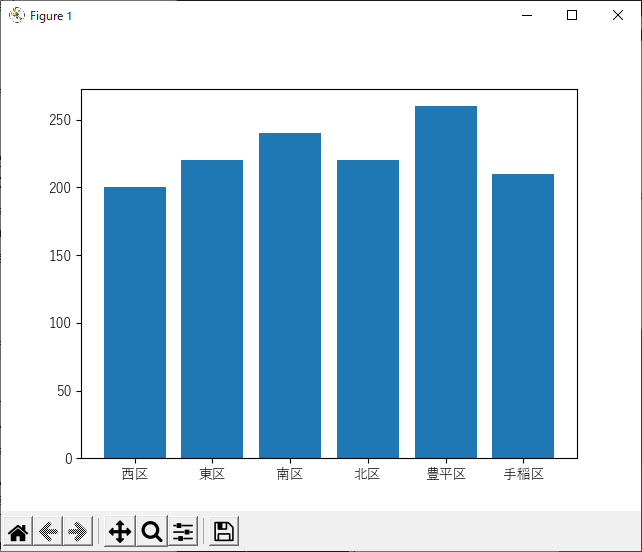
\includegraphics[width=7cm]{images/graph4.png} 

\end{legbox}
\end{pabox}


\section{numpy入門}
行列要素等の複数要素に対して効率よく処理をするためのライブラリがnumpyとなります。
\subsection{numpyの利用}

numpyライブラリの利用時のimportはasを使って「np」という別名を使うのが慣例となっています。

\begin{verbatim}
import numpy as np
\end{verbatim}


\begin{pabox}{numpy-1}
numpyを使ったデータ処理の一例を見てみましょう。
ここではリストとの違いを確認してみます。

\begin{legbox}{numpy1-1.py}
\begin{listing}{1}
import numpy as np

#listの生成
a = [ 1, 2, 3, 4, 5]
print(a)
#配列要素の生成
b = np.array([ 1, 2, 3, 4, 5])
print(b)
#listの長さが2倍
print( a * 2 )
#配列要素の中身がそれぞれ2倍
print( b * 2 )
#配列要素の要素同士が乗算される
print( b * b )
\end{listing}

実行結果\\
\begin{listing}{1}
[1, 2, 3, 4, 5]
[1 2 3 4 5]
[1, 2, 3, 4, 5, 1, 2, 3, 4, 5]
[ 2  4  6  8 10]
[ 1  4  9 16 25]
\end{listing}
\end{legbox}

\end{pabox}

\begin{pabox}{numpy-2}
numpyを使ったデータ生成の方法を見てみましょう。
ここでは関数(メソッド)を使った配列要素の生成方法を確認します。

\begin{legbox}{numpy1-2.py}
\begin{listing}{1}
import numpy as np

#rangeとよく似ていますが、整数以外も生成可能
print(np.arange(5))
print(np.arange(0, 2, 0.4))
#linspaceを使うと値を等分したリストを生成可能
print(np.linspace(0,100,5))
#10個の配列要素としての乱数を同時生成
print(np.random.rand(10))
\end{listing}

実行結果(例)\\
※乱数はそれぞれ出力される内容が異なります。\\
\begin{listing}{1}
[0 1 2 3 4]
[0.  0.4 0.8 1.2 1.6]
[  0.  25.  50.  75. 100.]
[0.61920954 0.29684569 0.94695251 0.79888711 0.77976444 0.10481961
 0.83043277 0.03716237 0.26022265 0.22519305]
\end{listing}
\end{legbox}

\end{pabox}

\newpage
\begin{pabox}{numpy-3}
numpyを使った条件判定を見てみましょう。
配列要素として乱数を生成し特定の値がいくつ含まれているか数えてみましょう。

\begin{legbox}{numpy1-3.py}
\begin{listing}{1}
import numpy as np

ransu = np.random.randint(1, 4, 10)
print(ransu)
#3のところを確認する
print(ransu == 3)
#3の数を数える
print(np.count_nonzero(ransu == 3))
\end{listing}

実行結果(例)\\
※乱数はそれぞれ出力される内容が異なります。\\
\begin{listing}{1}
[2 3 1 1 1 2 2 2 3 3]
[False  True False False False False False False  True  True]
3
\end{listing}
\end{legbox}

\end{pabox}

【高等学校情報科「情報1教員研修用教材(本編)】第3章で用いられている確定モデルと確率モデルに出てくるnumpyとmatplotlibについて今まで学習した内容と合わせて確認しましょう。
\newpage
\begin{pabox}{numpy-4}
参考資料「【高等学校情報科「情報1」教員研修用教材(本編)】第3章」139ページのサンプルプログラムを修正し、描画を見ながら確率モデルを確認しましょう。

\begin{legbox}{numpy1-4.py}
\begin{listing}{1}
import numpy as np # 整数をカウントするための関数呼び出し
import matplotlib.pyplot as plt # グラフプロットの呼び出し

for times in range(1,11):
    saikoro = np.random.randint(1, 6+1, 6 ** times) # サイコロを振る
    deme = [ ] # 出目の数を数える配列
    for i in range(6):
        deme.append(np.count_nonzero(saikoro==i+1)) 
  # 数を数えて配列に追加
    left = [1, 2, 3, 4, 5, 6] # グラフの左方向の値指定用
    plt.cla()
    plt.title("SAIKORO SIMULATION " + str(6 ** times) + " KAI") 
                    # グラフのタイトル
    plt.xlabel("ME") #X 軸のラベル
    plt.ylabel("KAISUU") #Y 軸のラベル
    plt.bar(left, deme, align="center") # グラフをプロット
    plt.draw() 
    plt.pause(2)
plt.show()
\end{listing}

実行結果\\

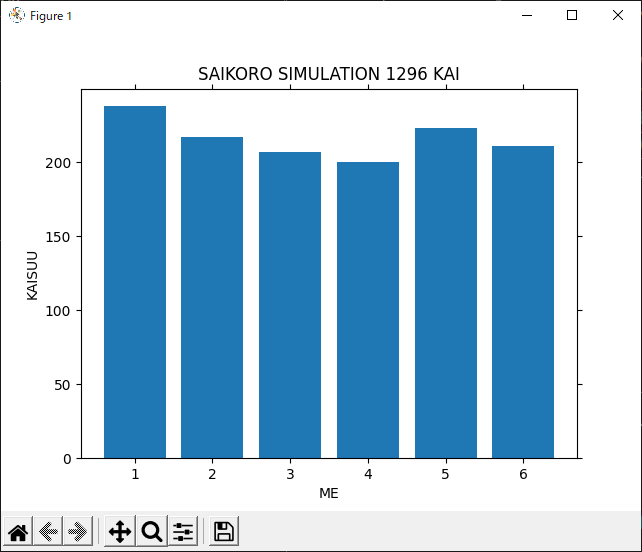
\includegraphics[width=5cm]{images/graph5.png} 

\end{legbox}


\end{pabox}

\begin{pabox}{numpy-5}
numpyとmatplotlibを使って三角関数のsinカーブを書いてみましょう。

コンピューター内部の角度は「°」ではなくradian単位を使うことが多いです。
0°から時計回り半周で円周率π(3.141592・・・・)となり、一周で2πとなるように表現される角度の単位です。

\begin{legbox}{numpy1-5.py}
\begin{listing}{1}
import numpy as np 
import matplotlib.pyplot as plt

#sinカーブの描画のための-180°~180までのradian設定
kakudo = np.linspace( -np.pi, np.pi, 361)
x = np.linspace(-180,180,361)
plt.plot(x, np.sin(kakudo))
plt.show()
\end{listing}

実行結果\\

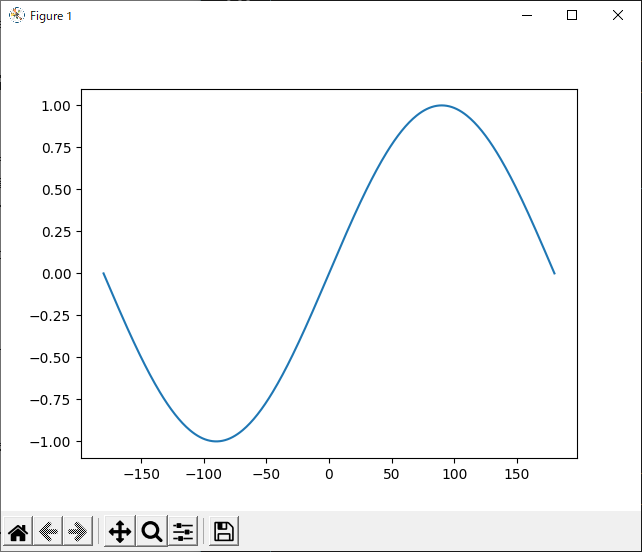
\includegraphics[width=6cm]{images/graph6.png} 

\end{legbox}


\end{pabox}
このような数値計算を効率よく行うためのライブラリがnumpyライブラリとなります。

\newpage
\section{WebAPIの利用}
ここではWebAPIによるJSONデータの取得を行い、グラフで視覚化してみます。

\subsection{外部JSONデータの読み込み}

まずはファイルに保存した外部JSONデータの読み込みを行い、データにアクセスしてみましょう。


\begin{pabox}{json1-1(JSONデータの読み込み)}
JSONデータをファイルとして保存してから読み込む方法を確認
\begin{legbox}{jsondatasimple.json}しましょう。
jsonファイルはコメントを記載できないので連想配列要素とリスト要素を確認しておいてください。
\begin{listing}{1}
{
    "class": "2年3組",
    "name": "佐々木",
    "score": [
        60,
        70,
        50,
        80,
        100
    ]
}
\end{listing}
\end{legbox}
jsonライブラリをimportし、jsonファイルをオープン後json.loadで読み込むことでdict型(連想配列)の値が取得されるので、左辺の変数に代入します。
\begin{legbox}{json1-1.py}
「jsondatasimple.json」を読み込んで各要素を取り出し、リストの合計を求めます。
\begin{listing}{1}
import json

jsonfile = open('jsondatasimple.json' , 'r', encoding='utf-8') 
#JSONデータ(dict型)として取り出す
loaded_data = json.load(jsonfile)  

#JSONデータのclass要素とname要素を取り出す
print(loaded_data['class'])
print(loaded_data['name'])

#JSONデータのscore要素のリストを取り出し合計を求める
total = 0
for x in loaded_data['score']:
    total = total + x

print("goukei = " + str(total))
\end{listing}
実行結果
\begin{listing}{1}
2年3組
佐々木
goukei = 360
\end{listing}

\end{legbox}
\end{pabox}

\subsection{WebAPIの利用}


WebAPIで公開されている政府や行政のデータは次のようなものがあります。

\begin{description}
	\item $https://www.e-stat.go.jp/$
	\item $https://data.pf-sapporo.jp/$
\end{description}

これらのデータを取得し利用する方法はurlを利用してjsonデータとしてダウンロードしdict型(連想配列)のデータとして読み込むことで可能となります。

今回利用するのは$https://ckan.pf-sapporo.jp/dataset/suikeijinkou$で取得できる札幌市の「将来推計人口の推移(平成17~47年)」です。

Excelでcsvファイルを読み込むと次の通りとなります。

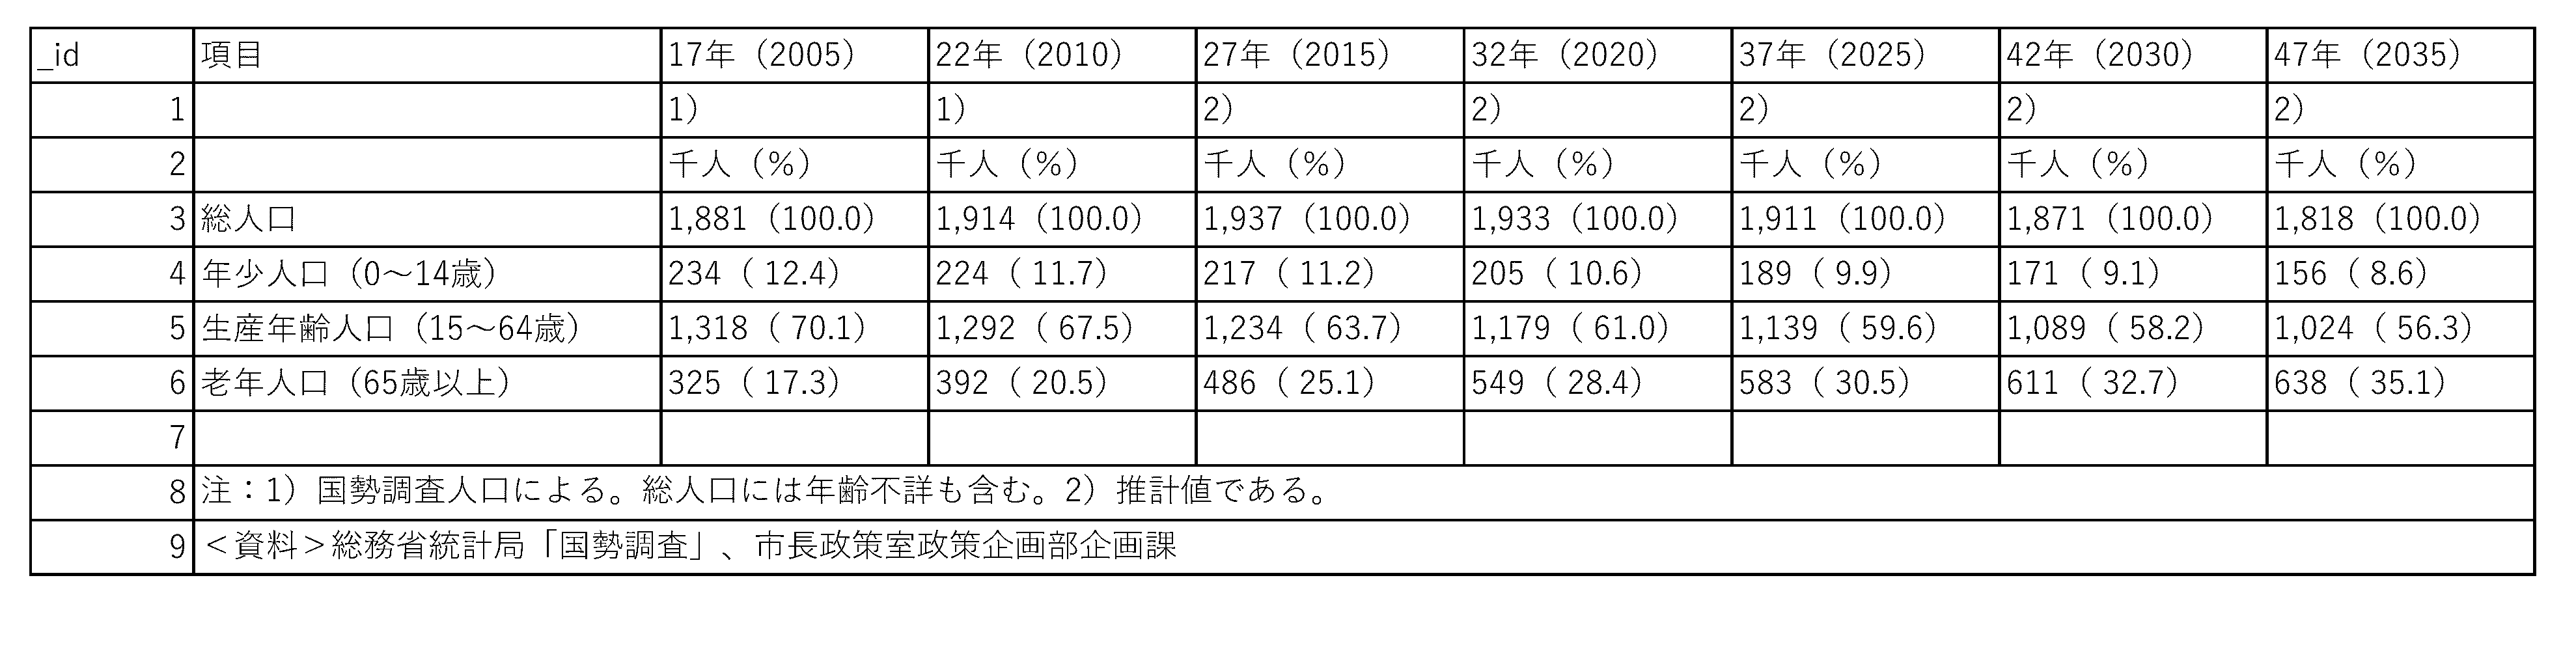
\includegraphics[width=14cm]{images/webapi1.png}

このデータをWebAPIによる読み込みをしてみましょう。

\begin{pabox}{webapi1-1(WebAPIによるJSONデータの読み込み)}
将来推計人口の推移(平成17~47年)のWebAPI用のURLからデータを読み込むプログラムです。
変数contentにdict型のデータとして取り込まれます。
\begin{legbox}{webapi1-1.py}
\begin{listing}{1}
import urllib
import urllib.request
import json

url = 'https://ckan.pf-sapporo.jp/api/3/action/datastore_search?
       resource_id=710b0236-6b28-441e-8500-f5c9be2e4c4a'
response = urllib.request.urlopen(url)
content = json.loads(response.read().decode('utf8'))

print(content)
\end{listing}
実行して結果を確認してください。
\end{legbox}
\end{pabox}



WebAPIで用いられるJSONによる文書構造の例は次の通りです。

\begin{grabox}{WebAPIで利用されるJSONの構造例}
\begin{listing}{1}
#辞書構造
{
    "help": --
    "success": --
    "result": {
        辞書構造
        "records":[
            リスト構造の中に辞書構造
        ],
        "fields":[
            リスト構造の中に辞書構造
        ],
        "_links":
            辞書構造
        "total": 9,
        "total_was_estimated": false
}
\end{listing}
\end{grabox}
それでは具体的にWebAPIのデータ構造を見てみましょう。

\begin{grabox}{JSON札幌市の将来推計人口の推移(平成17~47年)の抜粋}
\begin{listing}{1}
{
    "help": "https://ckan.pf-sapporo.jp/api/3/action/help_show?
       name=datastore_search",
    "success": true,
    "result": {
        "include_total": true,
        "limit": 100,
        "records_format": "objects",
        "resource_id": "710b0236-6b28-441e-8500-f5c9be2e4c4a",
        "total_estimation_threshold": null,
        "records": [
            {
                "_id": 1,
                "項目": "",
            ----省略----
            },
            {
                "_id": 2,
                "項目": "",
            ----省略----
            },
            {
                "_id": 3,
                "項目": "総人口",
                "17年(2005)": "1,881(100.0)",
                "22年(2010)": "1,914(100.0)",
                "27年(2015)": "1,937(100.0)",
                "32年(2020)": "1,933(100.0)",
                "37年(2025)": "1,911(100.0)",
                "42年(2030)": "1,871(100.0)",
                "47年(2035)": "1,818(100.0)"
            },
            {
                "_id": 4,
                "項目": "年少人口(0~14歳)",
            ----省略----
            },
            ----省略----
        ],
        "fields": [
            {
                "id": "_id",
                "type": "int"
            },
            {
                "id": "項目",
                "type": "text"
            },
            {
                "id": "17年(2005)",
                "type": "text"
            },
            {
                "id": "22年(20010)",
                "type": "text"
            },
            ----省略----
        ],
        "_links": {
            ----省略----
        },
        "total": 9,
        "total_was_estimated": false
    }
}
\end{listing}
\end{grabox}

このデータ構造からデータを取得する場合は

content辞書データからcontent["result"] で値を取り出すと"result"で参照されるdict型のデータが取得できます。

content["result"]からcontent["result"]["records"]で参照される辞書データ9個のリストデータが取得できます。(角カッコ「[]」で囲まれた要素はリストとして扱われます。)

これらのデータから総人口の推計を取り出すにはcontent["result"]["records"][2]を指定することで総人口の連想配列を取得することができます。
\begin{pabox}{webapi1-2(WebAPIによるJSONデータの読み込み)}
将来推計人口の推移(平成17~47年)のWebAPI用のURLからデータを読み込むプログラムです。
変数contentにdict型のデータとして取り込まれます。
\begin{legbox}{webapi1-2.py}
\begin{listing}{1}
import urllib
import urllib.request
import json

url = 'https://ckan.pf-sapporo.jp/api/3/action/datastore_search?
       resource_id=710b0236-6b28-441e-8500-f5c9be2e4c4a'
response = urllib.request.urlopen(url)
content = json.loads(response.read().decode('utf8'))


#値を取り出すための変数を用意
recode = content["result"]["records"][2]
#dictデータを順番に取り出す
for v in recode:
    print(v + ":" + str(recode[v]))
\end{listing}
実行結果
\begin{listing}{1}
_id:3
項目:総人口
17年(2005):1,881(100.0)
22年(2010):1,914(100.0)
27年(2015):1,937(100.0)
32年(2020):1,933(100.0)
37年(2025):1,911(100.0)
42年(2030):1,871(100.0)
47年(2035):1,818(100.0)
\end{listing}
値を取り出す13行目から16行目は次のようにitems()メソッドを利用してkeyと値を取り出すこともできます。
\begin{listing}{1}
recode = content["result"]["records"][2]
#recordのitems()メソッドでkeyと値をkとvに入れることができる
for k, v in recode.items():
    print(k + ":" + str(v))
\end{listing}
\end{legbox}
\end{pabox}

ここまでに取得したデータを使って推移および将来推計をグラフ化しましょう。

前述の「webapi1-3.py」の15,16行目の人口推計データを基にして数値に変換しmatplotlibに設定してみましょう。

\begin{pabox}{webapi1-3(WebAPIによるJSONデータの読み込み)}
将来推計人口の推移(平成17~47年)のWebAPI用のURLからデータを読み込むプログラムです。
変数contentにdict型のデータとして取り込まれます。
\begin{legbox}{webapi1-3.py}
\begin{listing}{1}
import urllib
import urllib.request
import json
import re
import matplotlib.pyplot as plt
import japanize_matplotlib

url = 'https://ckan.pf-sapporo.jp/api/3/action/datastore_search?
      resource_id=710b0236-6b28-441e-8500-f5c9be2e4c4a'
response = urllib.request.urlopen(url)
content = json.loads(response.read().decode('utf8'))

#値を取り出すための変数を用意
recode = content["result"]["records"][2]
#データラベルを初期化
label = []
#グラフデータを初期化
data = []

listdata = list(recode.items()) 
listdata.pop(0)
listdata.pop(0)
for k, v in listdata:
    l = re.search('[0-9]+年', k).group()
    label.append(l)
    v = v.replace(',','')
    n = int(re.search('[0-9]+', v).group())
    data.append(n*1000)
print(label, data)
x = [ 1, 2, 3, 4, 5, 6, 7 ]
plt.bar( x, data ,tick_label = label)

plt.show()
\end{listing}
\end{legbox}
\end{pabox}

もう一つ気象庁のデータを読み取り札幌エリアの天気概況を表示してみましょう。
\begin{pabox}{webapi1-4(WebAPIによるJSONデータの読み込み)}
気象庁の札幌エリアのデータを読み取り表示するプログラムを
\begin{legbox}{webapi1-4.py}
\begin{listing}{1}
import urllib
import urllib.request
import json
#詳細データ
url = 'https://www.jma.go.jp/bosai/forecast/data/forecast/
      016000.json'
#概況
url = 'https://www.jma.go.jp/bosai/forecast/data/
      overview_forecast/016000.json'
response = urllib.request.urlopen(url)
content = json.loads(response.read().decode('utf8'))

print(content["headlineText"])

\end{listing}
実行結果(ある日の結果)
\begin{verbatim}
空知地方では、29日は大雨による低い土地の浸水や河川の増水に、石狩・空知・後志地方では、29日は落雷や突風、ひょう、急な強い雨に
、30日にかけて濃い霧による交通障害に注意してください。
\end{verbatim}
\end{legbox}
\end{pabox}